\documentclass[unicode,11pt,a4paper,oneside,numbers=endperiod,openany]{scrartcl}
\usepackage{amsmath} 
\usepackage{amsfonts}
\usepackage{graphicx}
\usepackage{enumitem} 
\usepackage{longtable}
\usepackage{array}
\usepackage{xcolor}
\usepackage{booktabs}
\usepackage{multirow}
\usepackage{geometry}
\usepackage{listings}
\lstdefinestyle{mystyle}{
    basicstyle=\ttfamily\small,
    keywordstyle=\color{blue},
    commentstyle=\color{green},
    stringstyle=\color{red},
    numbers=left,
    numberstyle=\tiny,
    stepnumber=1,
    frame=single,
    breaklines=true,
    captionpos=b,
    tabsize=2
}

\lstdefinelanguage{MyC++}{
    language=C++,
    morekeywords={std, vector, string},
}

\lstdefinelanguage{MyPython}{
    language=Python,
    morekeywords={self},
}

\lstdefinelanguage{MyBatch}{
    morekeywords={echo, pause, set},
    sensitive=false, 
    morecomment=[l]{REM}, 
    morestring=[b]",
}

\lstdefinelanguage{MyBash}{
    basicstyle=\ttfamily,
    breaklines=true,
    frame=single,
    keywordstyle=\color{blue},
    commentstyle=\color{gray},
    showstringspaces=false
}
\usepackage{ifthen}
\usepackage[utf8]{inputenc}
\usepackage{graphics}
\usepackage{graphicx}
\usepackage{hyperref}

\pagestyle{plain}
\voffset -5mm
\oddsidemargin  0mm
\evensidemargin -11mm
\marginparwidth 2cm
\marginparsep 0pt
\topmargin 0mm
\headheight 0pt
\headsep 0pt
\topskip 0pt        
\textheight 255mm
\textwidth 165mm

\newcommand{\duedate} {}
\newcommand{\setduedate}[1]{%
\renewcommand\duedate {See iCorsi for due date}}
\newcommand\isassignment {false}
\newcommand{\setassignment}{\renewcommand\isassignment {true}}
\newcommand{\ifassignment}[1]{\ifthenelse{\boolean{\isassignment}}{#1}{}}
\newcommand{\ifnotassignment}[1]{\ifthenelse{\boolean{\isassignment}}{}{#1}}

\newcommand{\assignmentpolicy}{
\begin{table}[h]
\begin{center}
\scalebox{0.8} {%
\begin{tabular}{|p{0.02cm}p{16cm}|}
\hline
&\\
\multicolumn{2}{|c|}{\Large\textbf{HPC Lab ---  Submission Instructions}}\\
\multicolumn{2}{|c|}{\large\textbf{(Please, notice that following instructions are mandatory: }}\\
\multicolumn{2}{|c|}{\large\textbf{submissions that don't comply with, won't be considered)}}\\
&\\
\textbullet & Assignments must be submitted to \href{https://www.icorsi.ch}{iCorsi} (i.e. in electronic format).\\
\textbullet & Provide both executable package and sources (e.g. C/C++ files, Matlab). 
If you are using libraries, please add them in the file. Sources must be organized in directories called:\\
\multicolumn{2}{|c|}{\textit{Project\_number\_lastname\_firstname}}\\
& and  the  file must be called:\\
\multicolumn{2}{|c|}{\textit{project\_number\_lastname\_firstname.zip}}\\
\multicolumn{2}{|c|}{\textit{project\_number\_lastname\_firstname.pdf}}\\
\textbullet &  The TAs will grade your project by reviewing your project write-up, and looking at the implementation 
                 you attempted, and benchmarking your code's performance.\\

\textbullet & You are allowed to discuss all questions with anyone you like; however: (i) your submission must list anyone you discussed problems with and (ii) you must write up your submission independently.\\
\hline
\end{tabular}
}
\end{center}
\end{table}
}
\newcommand{\punkte}[1]{\hspace{1ex}\emph{\mdseries\hfill(#1~\ifcase#1{Points}\or{Points}\else{Points}\fi)}}


\newcommand\serieheader[6]{
\thispagestyle{empty}%
\begin{flushleft}

\includegraphics[width=0.4\textwidth]{usi_inf.png}
\end{flushleft}
  \noindent%
  {\large\ignorespaces{\textbf{#1}}\hspace{\fill}\ignorespaces{ \textbf{#2}}}\\ \\%
  {\large\ignorespaces #3 \hspace{\fill}\ignorespaces #4}\\
  \noindent%
  \bigskip
  \hrule\par\bigskip\noindent%
  \bigskip {\ignorespaces {\Large{\textbf{#5}}}
  \hspace{\fill}\ignorespaces \large \ifthenelse{\boolean{\isassignment}}{\duedate}{#6}}
  \hrule\par\bigskip\noindent%  \linebreak
 }

\makeatletter
\def\enumerateMod{\ifnum \@enumdepth >3 \@toodeep\else
      \advance\@enumdepth \@ne
      \edef\@enumctr{enum\romannumeral\the\@enumdepth}\list
      {\csname label\@enumctr\endcsname}{\usecounter
        {\@enumctr}%%%? the following differs from "enumerate"
	\topsep0pt%
	\partopsep0pt%
	\itemsep0pt%
	\def\makelabel##1{\hss\llap{##1}}}\fi}
\let\endenumerateMod =\endlist
\makeatother




\usepackage{textcomp}





\begin{document}


\setassignment

\serieheader{High-Performance Computing Lab}{Institute of Computing}{Student: Zitian Wang}{Discussed with: Ning Ding; Xiaorui Wang}{Solution for Project 4}{}
\newline

\assignmentpolicy



\section{Task: Ring maximum using MPI}
\begin{lstlisting}[language=MyC++, style=mystyle, caption={Ring sum function}]
  int main(int argc, char *argv[]) {

  // Initialize MPI, get size and rank
  int size, rank;
  MPI_Init(&argc, &argv);
  MPI_Comm_size(MPI_COMM_WORLD, &size);
  MPI_Comm_rank(MPI_COMM_WORLD, &rank);

  // IMPLEMENT: Ring sum algorithm
  int sum = rank; // initialize sum
  int rank_send = rank;
  int rank_recive;
  int send, receive;

  for (int i = 0; i < size - 1; i++){
    send = (rank + 1) % size;
    receive = (rank - 1 + size) % size;

    MPI_Sendrecv(
    &rank_send, 1, MPI_INT, send, 0, 
    &rank_recive, 1, MPI_INT, receive, 0, 
    MPI_COMM_WORLD, MPI_STATUS_IGNORE);

  sum += rank_recive;
  rank_send = rank_recive;
  }
  printf("Process %i: Sum = %i\n", rank, sum);
  // Finalize MPI
  MPI_Finalize();
  return 0;
}
\end{lstlisting}
To advoid deadlock issues, using \texttt{MPI\_Sendrecv} instead of \texttt{MPI\_Send} and \texttt{MPI\_Recv}.
\begin{lstlisting}[style=mystyle, language=MyBash, caption={Output of the Ring Program}]
    [wangzi@icsnode33 ring]$ mpirun ring_sum
    Process 0: Sum = 6
    Process 1: Sum = 6
    Process 2: Sum = 6
    Process 3: Sum = 6
\end{lstlisting}

\section{Task: Ghost cells exchange between neighboring processes}
\subsection{Cartesian two-dimensional MPI communicator}
\begin{lstlisting}[style=mystyle, language=MyC++, caption={Creating a Cartesian Communicator with Periodic Boundaries}]
    // TODO: set the dimensions of the processor grid and periodic boundaries in both dimensions
    dims[0] = 4;
    dims[1] = 4;
    periods[0] = 1;
    periods[1] = 1;

    // TODO: Create a Cartesian communicator (4*4) with periodic boundaries (we do not allow
    // the reordering of ranks) and use it to find your neighboring
    // ranks in all dimensions in a cyclic manner.
    MPI_Cart_create(MPI_COMM_WORLD, 2, dims, periods, 0, &comm_cart);
\end{lstlisting}

\subsection{derived data type}
\begin{lstlisting}[style=mystyle, language=MyC++, caption={Finding Neighbors and Creating a Derived Datatype}]
    // TODO: find your top/bottom/left/right neighbor using the new communicator, see MPI_Cart_shift()
    // rank_top, rank_bottom
    // rank_left, rank_right
    MPI_Cart_shift(comm_cart, 0, 1, &rank_top, &rank_bottom);
    MPI_Cart_shift(comm_cart, 1, 1, &rank_left, &rank_right);

    // part:1 start
    // TODO: create derived datatype data_ghost, create a datatype for sending the column, see MPI_Type_vector() and MPI_Type_commit()
    MPI_Type_vector(SUBDOMAIN, 1, DOMAINSIZE, MPI_DOUBLE, &data_ghost);
    MPI_Type_commit(&data_ghost);
\end{lstlisting}
\subsection{Exchange ghost cells}
\begin{lstlisting}[style=mystyle, language=MyC++, caption={Ghost Cell Exchange with Neighboring Cells in All Directions}]
    // TODO: ghost cell exchange with the neighbouring cells in all directions
    // Part 1: to the top
    MPI_Irecv(&data[1], DOMAINSIZE - 2, MPI_DOUBLE, rank_top, 0, comm_cart, &request);
    MPI_Send(&data[DOMAINSIZE + 1], DOMAINSIZE - 2, MPI_DOUBLE, rank_bottom, 0, comm_cart);
    MPI_Wait(&request, &status);

    // Part 2: to the bottom
    MPI_Irecv(&data[DOMAINSIZE * (DOMAINSIZE - 1) + 1], DOMAINSIZE - 2, MPI_DOUBLE, rank_bottom, 1, comm_cart, &request);
    MPI_Send(&data[DOMAINSIZE * (DOMAINSIZE - 2) + 1], DOMAINSIZE - 2, MPI_DOUBLE, rank_top, 1, comm_cart);
    MPI_Wait(&request, &status);

    // Define a custom MPI datatype for a ghost column
    MPI_Datatype data_ghost_column;
    MPI_Type_vector(SUBDOMAIN, 1, DOMAINSIZE, MPI_DOUBLE, &data_ghost_column);
    MPI_Type_commit(&data_ghost_column);

    // Part 3: to the left
    MPI_Irecv(&data[DOMAINSIZE], 1, data_ghost_column, rank_left, 2, comm_cart, &request);
    MPI_Send(&data[DOMAINSIZE + 1], 1, data_ghost_column, rank_right, 2, comm_cart);
    MPI_Wait(&request, &status);

    // Part 4: to the right
    MPI_Irecv(&data[2 * DOMAINSIZE - 1], 1, data_ghost_column, rank_right, 3, comm_cart, &request);
    MPI_Send(&data[2 * DOMAINSIZE - 2], 1, data_ghost_column, rank_left, 3, comm_cart);
    MPI_Wait(&request, &status);
\end{lstlisting}

\begin{lstlisting}[style=mystyle, language=MyBash, caption={Compilation and Execution of Ghost Communication}]
    [wangzi@icsnode33 ghost]$ make
    mpicc  ghost.c -o ghost
    [wangzi@icsnode33 ghost]$ mpirun -np 16 ./ghost
    data of rank 9 after communication
     9.0  5.0  5.0  5.0  5.0  5.0  5.0  9.0
     8.0  9.0  9.0  9.0  9.0  9.0  9.0 10.0
     8.0  9.0  9.0  9.0  9.0  9.0  9.0 10.0
     8.0  9.0  9.0  9.0  9.0  9.0  9.0 10.0
     8.0  9.0  9.0  9.0  9.0  9.0  9.0 10.0
     8.0  9.0  9.0  9.0  9.0  9.0  9.0 10.0
\end{lstlisting}
    
\subsection{Bonus}

\begin{lstlisting}[style=mystyle, language=MyC++, caption={Exchanging Ghost Values with Ordinal Neighbors}]
    // Bonus [10 Points]: Also exchange ghost values with the neighbors in ordinal directions (northeast, southeast, southwest and northwest).
    int coords[2]; 
    int coords_nw[2], coords_ne[2], coords_sw[2], coords_se[2];
    int rank_northwest, rank_northeast, rank_southwest, rank_southeast; 
    MPI_Cart_coords(comm_cart, rank, 2, coords);
    coords_nw[0] = (coords[0] - 1 + dims[0]) % dims[0];
    coords_nw[1] = (coords[1] - 1 + dims[1]) % dims[1];
    MPI_Cart_rank(comm_cart, coords_nw, &rank_northwest);

    coords_ne[0] = (coords[0] - 1 + dims[0]) % dims[0];
    coords_ne[1] = (coords[1] + 1) % dims[1];
    MPI_Cart_rank(comm_cart, coords_ne, &rank_northeast);

    coords_sw[0] = (coords[0] + 1) % dims[0];
    coords_sw[1] = (coords[1] - 1 + dims[1]) % dims[1];
    MPI_Cart_rank(comm_cart, coords_sw, &rank_southwest);

    coords_se[0] = (coords[0] + 1) % dims[0];
    coords_se[1] = (coords[1] + 1) % dims[1];
    MPI_Cart_rank(comm_cart, coords_se, &rank_southeast);
    MPI_Sendrecv(&data[DOMAINSIZE + 1], 1, MPI_DOUBLE, rank_southeast, 4,
                 &data[0], 1, MPI_DOUBLE, rank_northwest, 4,
                 comm_cart, &status);

    MPI_Sendrecv(&data[DOMAINSIZE + DOMAINSIZE - 2], 1, MPI_DOUBLE, rank_southwest, 5,
                 &data[DOMAINSIZE - 1], 1, MPI_DOUBLE, rank_northeast, 5,
                 comm_cart, &status);

    MPI_Sendrecv(&data[(DOMAINSIZE - 2) * DOMAINSIZE + 1], 1, MPI_DOUBLE, rank_northeast, 6,
                 &data[DOMAINSIZE * (DOMAINSIZE - 1)], 1, MPI_DOUBLE, rank_southwest, 6,
                 comm_cart, &status);

    MPI_Sendrecv(&data[(DOMAINSIZE - 2) * DOMAINSIZE + DOMAINSIZE - 2], 1, MPI_DOUBLE, rank_northwest, 7,
                 &data[DOMAINSIZE * DOMAINSIZE - 1], 1, MPI_DOUBLE, rank_southeast, 7,
                 comm_cart, &status);
\end{lstlisting}

\begin{lstlisting}[style=mystyle, language=MyBash, caption={Output of Ghost Cell Communication}]
    [wangzi@icsnode35 ghost]$ mpirun -np 16 ./ghost
    data of rank 9 after communication
     4.0  5.0  5.0  5.0  5.0  5.0  5.0  6.0
     8.0  9.0  9.0  9.0  9.0  9.0  9.0 10.0
     8.0  9.0  9.0  9.0  9.0  9.0  9.0 10.0
     8.0  9.0  9.0  9.0  9.0  9.0  9.0 10.0
     8.0  9.0  9.0  9.0  9.0  9.0  9.0 10.0
     8.0  9.0  9.0  9.0  9.0  9.0  9.0 10.0
     8.0  9.0  9.0  9.0  9.0  9.0  9.0 10.0
    12.0 13.0 13.0 13.0 13.0 13.0 13.0 14.0
\end{lstlisting}
    


\section{Task: Parallelizing the Mandelbrot set using MPI}
\subsection{update functions createPartition, updatePartition and createDomain}
\begin{lstlisting}[style=mystyle, language=MyC++, caption={Cartesian Partition Creation}]
    Partition createPartition(int mpi_rank, int mpi_size) {
        Partition p;
    
        // TODO: determine size of the grid of MPI processes (p.nx, p.ny), see MPI_Dims_create()
        int dims[2];
        MPI_Dims_create(mpi_size, 2, dims);
        p.ny = dims[1];
        p.nx = dims[0];
    
        // TODO: Create cartesian communicator (p.comm), we do not allow the reordering of ranks here, see MPI_Cart_create()
        int periods[2] = {0, 0};
        MPI_Comm comm_cart;
        MPI_Cart_create(MPI_COMM_WORLD, 2, dims, periods, 0, &comm_cart);
        p.comm = comm_cart;
        
        // TODO: Determine the coordinates in the Cartesian grid (p.x, p.y), see MPI_Cart_coords()
        int coords[2];
        MPI_Cart_coords(p.comm, mpi_rank, 2, coords);
        p.x = coords[0];
        p.y = coords[1];
    
        return p;
    }
\end{lstlisting}

\begin{lstlisting}[style=mystyle, language=MyC++, caption={Updating Cartesian Partition Coordinates}]
    Partition updatePartition(Partition p_old, int mpi_rank) {
        Partition p;
    
        // copy grid dimension and the communicator
        p.ny = p_old.ny;
        p.nx = p_old.nx;
        p.comm = p_old.comm;
        
        // TODO: update the coordinates in the cartesian grid (p.x, p.y) for given mpi_rank, see MPI_Cart_coords()
        int coords[2];
        MPI_Cart_coords(p.comm, mpi_rank, 2, coords);
        p.x = coords[0];
        p.y = coords[1];
    
        return p;
    }
\end{lstlisting}

\begin{lstlisting}[style=mystyle, language=MyC++, caption={Creating a Local Domain}]
    Domain createDomain(Partition p) {
        Domain d;
        
        // TODO: compute size of the local domain
        d.nx = IMAGE_WIDTH / p.nx;
        d.ny = IMAGE_HEIGHT / p.ny;
    
        if (p.x == p.nx - 1) {
            d.nx += IMAGE_WIDTH % p.nx;
        }
        if (p.y == p.ny - 1) {
            d.ny += IMAGE_HEIGHT % p.ny;
        }
        
        // TODO: compute index of the first pixel in the local domain
        d.startx = p.x * (IMAGE_WIDTH / p.nx);
        d.starty = p.y * (IMAGE_HEIGHT / p.ny);
    
        // TODO: compute index of the last pixel in the local domain
        d.endx = d.startx + d.nx - 1;
        d.endy = d.starty + d.ny - 1;
    
        return d;
    }
\end{lstlisting}

\subsection{Send the data to the master}
\begin{lstlisting}[style=mystyle, language=MyC++, caption={Sending and Receiving Local Partition Data}]
    // TODO: send local partition c to the master process
    MPI_Send(c, d.nx * d.ny, MPI_INT, 0, 0, MPI_COMM_WORLD); 
    // TODO: receive partition of the process proc into array c (overwrite its data)
    MPI_Recv(c, d1.nx * d1.ny, MPI_INT, proc, 0, MPI_COMM_WORLD, MPI_STATUS_IGNORE);
\end{lstlisting}

\begin{figure}[h]
    \centering
    
\includegraphics[width=0.5\textwidth]{pictures/mandel.png}
    \caption{Mandelbrot set}
\end{figure}

\subsection{Performance observe}
\begin{figure}[h]
    \centering
    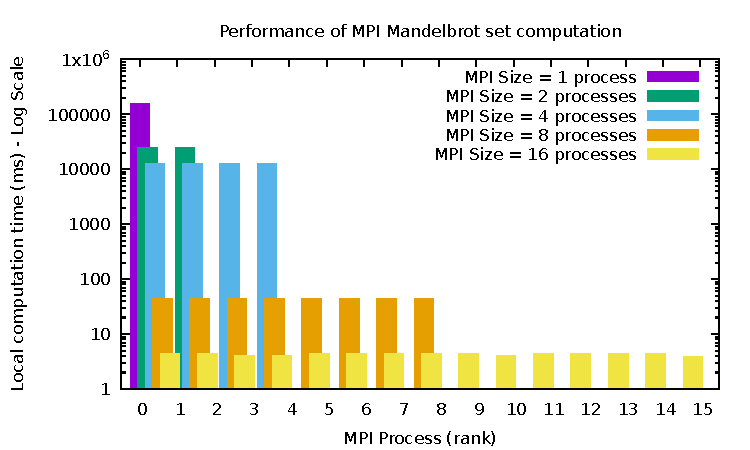
\includegraphics[width=0.9\textwidth]{pictures/perf.pdf}
    \caption{Performance Report}
\end{figure}
The highest computation times are visible for the smaller number of processes (MPI size = 1 and 2), which significantly decrease as the number of processes increases. This decrease flattens somewhat for higher numbers of processes (MPI size = 8 and 16), indicating a diminishing return in performance gains. The graph shows expected scalability up to a point, where adding more processes yields lesser improvements in performance, likely due to overhead associated with managing more processes and increased communication between them.


Blocking \texttt{MPI\_Send} and \texttt{MPI\_Recv} calls can lead to waiting if one process is delayed. Replace them with \texttt{MPI\_Isend} and \texttt{MPI\_Irecv}. Besides, each process is single-threaded, so using vectorized instructions (SIMD) and multithreading (OpenMP) can also help for enhance performance.

\section{Task: Parallel matrix-vector multiplication and the power method}
\begin{lstlisting}[style=mystyle, language=MyC++, caption={Broadcasting and Preparing for MPI\_Allgatherv}]
    // To do: Broadcast the random initial guess vector to all MPI processes.
    // Hint: MPI_Bcast.
    MPI_Bcast(y, n, MPI_DOUBLE, 0, MPI_COMM_WORLD);
  
    // Prepare for MPI_Allgatherv
    int* recvcounts = (int*)malloc(size * sizeof(int));
    int* displs = (int*)malloc(size * sizeof(int));
  
    for (int i = 0; i < size; ++i) {
      if (i < remainder) {
        recvcounts[i] = nrows_base + 1;
        displs[i] = i * recvcounts[i];
      } else {
        recvcounts[i] = nrows_base;
        displs[i] = i * nrows_base + remainder;
      }
    }
\end{lstlisting}
\newpage
\begin{lstlisting}[style=mystyle, language=MyC++, caption={Determining Local Row Ranges for MPI Processes}]
    int nrows_base = n / size;       // Base number of rows per process
    int remainder = n % size;        // Extra rows to distribute
    int nrows_local;
    int row_beg_local;
    int row_end_local;
  
    if (rank < remainder) {
      nrows_local = nrows_base + 1;
      row_beg_local = rank * nrows_local;
    } else {
      nrows_local = nrows_base;
      row_beg_local = rank * nrows_base + remainder;
    }
    row_end_local = row_beg_local + nrows_local - 1;
  
    printf("[Proc %3d] Doing rows %d to %d\n", rank, row_beg_local, row_end_local);
\end{lstlisting}
  
\begin{figure}[h]
    \centering
    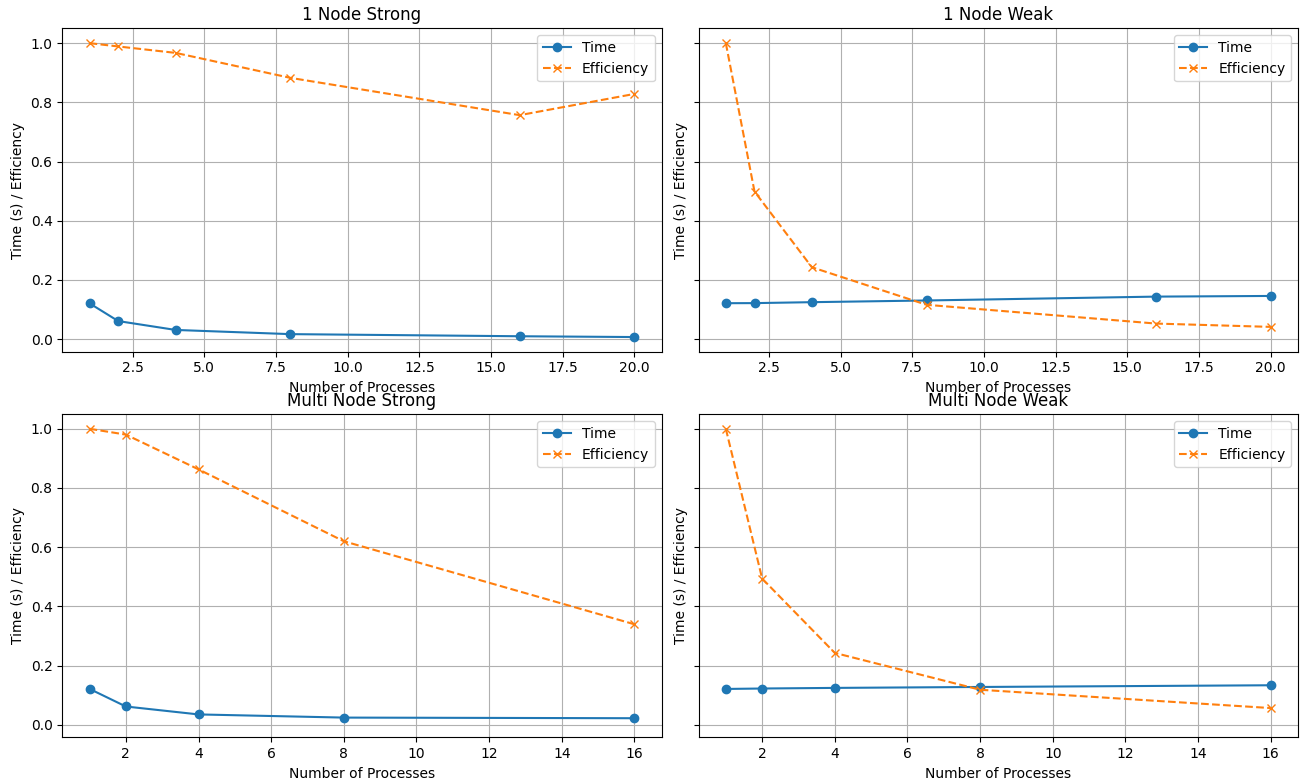
\includegraphics[width=1\textwidth]{pictures/report.png}
    \caption{Analysis Report}
\end{figure}

In our MPI scalability tests, we focused on the time to solution and efficiency across different configurations and scaling strategies. Notably, in strong scaling on a single node, the time to solution improved significantly as we increased the number of processors from 1 to 20. For instance, it decreased from 0.121156 seconds with one processor to just 0.007312 seconds with 20 processors, showcasing a dramatic improvement in performance.

However, this scaling efficiency tends to decrease as we add more processors. While ideal efficiency would be close to 1, the overhead from communication and synchronization among processors dampens this figure. This is especially pronounced when expanding to multiple nodes, where the time to solution slightly worsens due to inter-node communication. For example, with 16 processors spread across different nodes, the efficiency is lower compared to them being on a single node.

For weak scaling, where the problem size grows with the square root of the number of processors, we noticed that the time to solution remains relatively stable, indicating a well-balanced load among processors. However, as we extend to multiple nodes, such as moving from 1 to 16 processors, slight increases in execution times from 0.121217 to 0.133656 seconds suggest emerging bottlenecks in network communication and data management.

These results underline the importance of considering both algorithmic and system architecture optimizations. Enhancing communication patterns and refining problem partitioning strategies could further improve our application's scalability and efficiency.


\end{document}
